%\documentclass[journal]{vgtc}                % final (journal style)
\documentclass[review,journal]{vgtc}         % review (journal style)
%\documentclass[widereview]{vgtc}             % wide-spaced review
%\documentclass[preprint,journal]{vgtc}       % preprint (journal style)
%\documentclass[electronic,journal]{vgtc}     % electronic version, journal

%% Uncomment one of the lines above depending on where your paper is
%% in the conference process. ``review'' and ``widereview'' are for review
%% submission, ``preprint'' is for pre-publication, and the final version
%% doesn't use a specific qualifier. Further, ``electronic'' includes
%% hyperreferences for more convenient online viewing.

%% Please use one of the ``review'' options in combination with the
%% assigned online id (see below) ONLY if your paper uses a double blind
%% review process. Some conferences, like IEEE Vis and InfoVis, have NOT
%% in the past.

%% Please note that the use of figures other than the optional teaser is not permitted on the first page
%% of the journal version.  Figures should begin on the second page and be
%% in CMYK or Grey scale format, otherwise, colour shifting may occur
%% during the printing process.  Papers submitted with figures other than the optional teaser on the
%% first page will be refused.

%% These three lines bring in essential packages: ``mathptmx'' for Type 1
%% typefaces, ``graphicx'' for inclusion of EPS figures. and ``times''
%% for proper handling of the times font family.

\usepackage{url}
\usepackage{mathptmx}
\usepackage{graphicx}
\usepackage{times}
%\usepackage{egweblnk}
\usepackage{cite}
\usepackage[usenames,dvipsnames,svgnames]{xcolor}
\usepackage{subfigure}
\usepackage{flushend}
\usepackage[compact]{titlesec}
\usepackage[normalem]{ulem}

%% We encourage the use of mathptmx for consistent usage of times font
%% throughout the proceedings. However, if you encounter conflicts
%% with other math-related packages, you may want to disable it.

%% This turns references into clickable hyperlinks.
\usepackage[bookmarks,backref=true,linkcolor=black]{hyperref} %,colorlinks
\hypersetup{
  pdfauthor = {},
  pdftitle = {},
  pdfsubject = {},
  pdfkeywords = {},
  colorlinks=true,
  linkcolor= black,
  citecolor= black,
  pageanchor=true,
  urlcolor = black,
  plainpages = false,
  linktocpage
}

% Spacing tricks
\setlength{\baselineskip}{9pt}
\setlength{\belowcaptionskip}{-0.4cm}
\setlength{\abovecaptionskip}{3pt}
%\setlength{\parskip}{0pt}
%\titlespacing*{\section}{0pt}{1ex}{1ex}
%\titlespacing*{\subsection}{0pt}{1ex}{1ex}
\titlespacing*{\subsubsection}{0pt}{1ex}{1ex}
%\setlength{\intextsep}{0pt}

\def\etal{\textit{et al.}}
\renewcommand\floatpagefraction{1.0}
\renewcommand\topfraction{1.0}
\renewcommand\bottomfraction{.9}
\renewcommand\textfraction{.1}
\setcounter{totalnumber}{20}
\setcounter{topnumber}{10}
\setcounter{bottomnumber}{10}
\definecolor{MyGreen}{rgb}{0,0.7,0}
\definecolor{MyWhite}{rgb}{1,1,1}
\definecolor{MyGray}{rgb}{0.5,0.5,0.5}
\definecolor{LightGray}{rgb}{0.7,0.7,0.7}
\definecolor{DarkGray}{rgb}{0.3,0.3,0.3}
\definecolor{DarkYellow}{rgb}{0.7,0.7,0.0}
\definecolor{MyNavyBlue}{rgb}{0.2,0.3,0.7}
\definecolor{darkgreen}{rgb}{0,0.55,0}
\newcommand{\black}[1]{{\color{Black} #1}}
\newcommand{\white}[1]{{\color{MyWhite} #1}}
\newcommand{\gray}[1]{{\color{MyGray} #1}}
\newcommand{\red}[1]{{\color{red} #1}}
\newcommand{\green}[1]{{\color{MyGreen} #1}}
\newcommand{\blue}[1]{{\color{MyNavyBlue} #1}}
\newcommand{\yellow}[1]{{\color{DarkYellow} #1}}
\newcommand{\maybe}[1]{\yellow{#1}}
\newcommand{\rout}[1]{\red{\sout{#1}}}
\newcommand{\repl}[2]{\rout{#1} \green{#2}}
\newcommand{\fix}[1]{\red{\emph{(#1)}}}
\newcommand{\Fix}[1]{\begin{itemize} \renewcommand\labelitemi{\red{--}} \item \red{#1} 
\end{itemize}}

\newcommand{\todo}[1] {\textbf{[~}\textcolor {red}{#1}\marginpar{\textcolor {red}{\centerline{{\Huge \textbf{!}}}}}\textbf{~]}}
\newcommand{\question}[1] {\textbf{[~}\textcolor {darkgreen}{#1}\marginpar{\textcolor {darkgreen}{\centerline{{\Huge \textbf{!}}}}}\textbf{~]}}
\newcommand{\diff}[1]{[\textcolor{blue}{#1}\marginpar{\textcolor{blue}{\centerline{{\Huge \textbf{!}}}}}]}

\setlength\fboxsep{0pt}

\def\IC{IC}
\def\SAR{SAR}
\def\USAR{USAR}


%% If you are submitting a paper to a conference for review with a double
%% blind reviewing process, please replace the value ``0'' below with your
%% OnlineID. Otherwise, you may safely leave it at ``0''.
\onlineid{249}

%% declare the category of your paper, only shown in review mode
\vgtccategory{System}

%% allow for this line if you want the electronic option to work properly
\vgtcinsertpkg

%% In preprint mode you may define your own headline.
%\preprinttext{To appear in an IEEE VGTC sponsored conference.}

%%%%%%%%%%%%%%%%%%%%%%%%%%%%%%%%%%%%%%%%%%%%%%%%%%%%%%%%%%%%%%%%%%%%%%%%%%%%%%%%%%%%%%%%%%%
%%%%%%%%%%%%%%%%%%%%%%%%%%%%%%%%%%%%%%%%%%%%%%%%%%%%%%%%%%%%%%%%%%%%%%%%%%%%%%%%%%%%%%%%%%%

%% Paper title.
%\title[Decision-Support for Search \& Rescue Planning]{Decision-Support for Urban Search \& Rescue Mission Planning through Visualization-Based Analysis}
\title{Decision-Support for Urban Search \& Rescue Mission Planning\\ through Visualization-Based Analysis}

% @Alex B.: Has the author order of Jonas & Alex K. been discussed with them?
\author{Alexander Bock, Jonas Lundberg, Alexander Kleiner, and Timo Ropinski}
\authorfooter{
    \item Alexander Bock and Timo Ropinski are with the Scientific Visualization Group, Link\"oping University. e-mail: \{alexander.bock\textbar timo.ropinski\}@liu.se
    \item Jonas Lundberg is with the Graphic Design Group, Link\"oping University. e-mail: jonas.lundberg@liu.se
    \item Alexander Kleiner is with the Collaborative Robotics Group, Link\"oping University. e-mail: alexander.kleiner@liu.se
}

\shortauthortitle{Bock \etal: Urban Search \& Rescue Mission Planning}

\teaser{
	\centering
	\subfigure[Voxelized 3D point cloud rendering enabling the operator to form an increased awareness of a damaged office building.]{
		\fbox{\includegraphics[height=0.25\linewidth]{figures/image1.jpg}}\label{fig:teaser:1}
	}
	\hfill
	\subfigure[Viable paths through office buildings of the Tohoku university with two hazardous environments highlighted.]{
		\fbox{\includegraphics[height=0.25\linewidth]{figures/image2.jpg}}\label{fig:teaser:2}
	}
	\hfill
	\subfigure[Top-down view of the area providing contextual information.]{
		\fbox{\includegraphics[height=0.25\linewidth]{figures/image2-overview.jpg}}\label{fig:teaser:3}
	}
	\hfill
	\subfigure[In-depth analysis of a path ensemble using parallel coordinates plots and profile plots.]{
		\fbox{\includegraphics[height=0.25\linewidth]{figures/pcpprofile.png}}\label{fig:teaser:4}
	}
  \caption{Our proposed visualization system applied to path planning at the a collapsed building at Tohoku university. Different views (a--c) present the operator with a comprehensive understanding of the building, allowing him to select and inspect paths that reach a point of interest. The assessment of the trade-off between the paths is supported by a set of interactive visual analysis tools (d).\vspace*{0.3cm}}
  \label{fig:teaser}
}


\abstract{
We propose a visualization system for incident commanders in urban search~\&~rescue scenarios that supports access path planning for post-disaster structures. Utilizing point cloud data acquired from unmanned robots, we combine visualization with visual analytics methods to allow for assessment of automatically generated paths. Data uncertainty and a priori unknown information make fully automated systems impractical for this problem and call for interaction with an expert user. To this end, we present a set of viable access paths, whose computation is based on varying risk factors, to the incident commander in a 3D environment combined with the visual analysis tools to inspect paths in detail and make informed decisions and trade-offs. Based on these decisions, a responder is guided along the path by the incident commander, who can interactively annotate and reevaluate the acquired point cloud to react to the dynamics of the situation. We describe design considerations for our system, its technical realization, and discuss the results of an expert evaluation, which we conducted to assess the usefulness of our system.
}

%% Keywords that describe your work. Will show as 'Index Terms' in journal
%% please capitalize first letter and insert punctuation after last keyword
\keywords{Urban search~\&~rescue mission planning, decision support, visual analysis.}

%% ACM Computing Classification System (CCS). 
%% See <http://www.acm.org/class/1998/> for details.
%% The ``\CCScat'' command takes four arguments.

\CCScatlist{ % not used in journal version
   \CCScat{I.3.7}{Computer Graphics}{Three-Dimensional Graphics and Realism}{Color, shading, shadowing, and texture}
}

%% Uncomment below to disable the manuscript note
%\renewcommand{\manuscriptnotetxt}{}

%% Copyright space is enabled by default as required by guidelines.
%% It is disabled by the 'review' option or via the following command:
% \nocopyrightspace

%%%%%%%%%%%%%%%%%%%%%%%%%%%%%%%%%%%%%%%%%%%%%%%%%%%%%%%%%%%%%%%%%%%%%%%%%%%%%%%%%%%%%%%%%%%
%%%%%%%%%%%%%%%%%%%%%%%%%%%%%%%%%%%%%%%%%%%%%%%%%%%%%%%%%%%%%%%%%%%%%%%%%%%%%%%%%%%%%%%%%%%

\begin{document}

\firstsection{Introduction}

\maketitle

\vspace{-0.15cm}

Natural and man-made disasters causing structural damage to inhabited buildings are an ever-present danger. As time-to-rescue is one of the most important factors that determines victims' survivability, it is of highest importance for the rescue responders to reach victims as fast as possible in order to provide medical attention or extraction. Planning and executing optimal paths through buildings is, however, difficult as structural damage makes available floor plans outdated. Furthermore, structural weaknesses as well as hazardous environments, can make localized regions or whole areas inaccessible. While trained responders can use their knowledge and intuition to spot these hazards, it is paramount that the \emph{Incident Commander} (IC), who has global information about the building, can analyze the information and coordinate multiple rescue responders. Naturally, computer support systems involving expert users can help to tackle this challenge. In order to design a system that effectively amplifies human decision-making, it is vital to consider how decisions in dynamic unpredictable situations are made~\cite{Lundberg2012}. The system can then be designed to support planning based on experience, to increase quality of control, and to support decision-making, not only with regard to expected decisions, but also considering unexpected developments.

There are well-defined protocols in place to describe the actions taken during an \emph{Urban Search~\&~Rescue} (USAR) operation. The Federal Emergency Management Agency describes five steps that are performed by the rescue team~\cite{fema08}. During the assessment step, 2D maps of the collapsed building are hand-drawn, based on the descriptions of rescue responders who are moving within the building searching for victims. In this exploration phase, they might stumble into hazardous areas, for example gas leaks, that endanger the rescuer's life. Even though the guidelines require these sketches to include a cross section of the building, a drawing of an unstructured 3D building is inaccurate and ineffective to construct a comprehensive mental model, yet this is the currently employed technique.

In recent years, technological developments made it possible to use ground-based unmanned vehicles to perform the initial exploration. The robots can be deployed into the building and are equipped with sensors that can detect victims, gather information about potentially hazardous environments, and perform detailed scans of rooms to create a 3D point cloud of the building's interior. These unstructured point clouds are collated and co-registered in real-time to produce a consistent map of the building. Using simultaneous localization and mapping algorithms (SLAM)~\cite{Dissanayake01asolution, Ziparo459917}, these maps are used by the robots to navigate buildings while exploring accessible areas. After the map has been acquired, the \IC\ can analyze the collected data and plan viable access paths for the rescue responders that enter the building to reach certain \emph{Points of Interest} (POIs). In most cases, these POIs are potential locations of victims, but they can also be other mission critical areas that need to be reached and analyzed.

In this paper, we propose a visualization system that uses the acquired and annotated map during USAR missions to support access path planning. The system preprocesses the point cloud data to create an interactive 3D rendering that is tailored to increase the commander's spatial awareness of the internal structures (see Figure~\ref{fig:teaser}~(a-c)) and further support the analysis and planning of viable access paths (see Figure~\ref{fig:teaser}~(d)). The spatial knowledge is paramount in detecting the location of unreachable areas, so-called voids, a prime location where victims might be trapped. The gathered information is used to instruct rescue responders to reach several POIs and the \IC\ can annotate the visualization with new real-time information that he receives from the on-site rescue responders, thus shifting the decision making process from being opportunistic to being strategical. Based on the available information, our system computes an ensemble of possible access paths from the entry point to the POIs, where each path is based on varying risk factors, for example overall distance, closest distance to a hazard, or the structural stability of the ground underneath. Uncertainty in the data and a priori unknown information make it infeasible to employ fully automatic algorithms to detect the globally optimal path. Thus, our system supports the \IC\ in the process of analyzing and comparing all available paths at once to reach a conclusion which minimizes the rescuer's danger and travel time.

%%%%%%%%%%%%%%%%%%%%%%%%%%%%%%%%%%%%%%%%%%%%%%%%%%%%%%%%%%%%%%%%%%%%%%%%%%%%%%%%%%%%%%%%%%%
%%%%%%%%%%%%%%%%%%%%%%%%%%%%%%%%%%%%%%%%%%%%%%%%%%%%%%%%%%%%%%%%%%%%%%%%%%%%%%%%%%%%%%%%%%%

%\vspace*{-3pt}
\section{Related Work} \label{sec:relatedwork}
\noindent {\bfseries Emergency management.} Much of the visualization-oriented work published in the field of emergency management is concerned with evacuation planning well before any rescue operation has to be performed. Notable work was performed by Reddy~\etal, which enables analyzing possible bottlenecks of escape routes~\cite{EuroVA12:13-17:2012}. While algorithms from these areas could be utilized to our benefit, they usually assume perfect walking conditions and a constant structural layout of the building. Ribarsky~\etal\ presented a system organizing first responders in intact structures~\cite{Ribarsky:2010}. Kim~\etal\ developed a system enhancing the situational awareness of responders using a mobile visual analytics tool~\cite{Kim:2008}. Another related area is the research on visual analysis-supported ensemble steering. While these techniques use ensembles and visualization to reduce the impact of uncertainty in the input parameters, our system helps the operator to find the best trade-off between the various runs. Ribi\v{c}i\'c~\etal\ investigated steering ensembles of flooding simulations using visual analysis~\cite{6280550}. They showed that visual analysis is a useful method for experts to interpret this kind of data. Their idea of generating different measures about a particular flooding scenario inspired our approach to compute path ensembles. 

Many existing planning systems deployed nowadays in USAR scenarios are based on 2D representations~\cite{kleiner_et_al_ssrr09,KohlbrecherMeyerStrykKlingaufFlexibleSlamSystem2011,Pellenz2009SMU}. Given the 2D map of the environment, one common approach to path planning is to plan the shortest trajectory and to follow this trajectory stepwise. In harsh environments, however, the safest path, not the shortest, may be desirable. Wirth~\etal\ introduced an exploration strategy and path planner that utilizes occupancy grid maps when planning to reach several targets at the same time~\cite{Wirth2007ETA1}. Consequently, the method selects the safest alternative consisting of target location and the corresponding path. Preliminary extensions towards exploration in 3D with regard to detection of voids were introduced by Dornhege and Kleiner~\cite{dornhege2011frontier}.

%\noindent\textbf{Visual analytics.} There has been work investigating the sense-making process when using visual analytics tools. Gotz \etal\ investigated how to measure insight provenance, a critical measure to judge the quality of reasoning~\cite{Gotz2009}. Roberts presented a state-of-the-art report on how to apply the visual analytics models and techniques using coordinated and multiple views~\cite{roberts2007multipleviews}. Keim \etal\ provide a good overview about the current developments in the field~\cite{keim2010mastering}.

\noindent {\bfseries Point cloud visualization.} As the real-time availability of high resolution point clouds has increased in recent years, there has been much research on rendering techniques for this kind of data. Basic rendering capabilities are provided by the widely used Point Cloud Library, which provides a wide array of functionality~\cite{Rusu11ICRA}. Furthermore, there has been work by Richter~\etal\ using a level-of-detail structure to render massive point clouds at high frame rates~\cite{Richter:2010:ORV:1811158.1811178}. Xu~\etal\ showed that non-photorealistic rendering techniques can be applied to point cloud data~\cite{conf/npar/XuC04}. The contour lines in their rendering inspired our rendering algorithm. More recently, Pintus~\etal\ presented a rendering algorithm that enhances features of unstructured point clouds in real-time without preprocessing~\cite{Pintus:2011:RRM:2384495.2384513}.

%%%%%%%%%%%%%%%%%%%%%%%%%%%%%%%%%%%%%%%%%%%%%%%%%%%%%%%%%%%%%%%%%%%%%%%%%%%%%%%%%%%%%%%%%%%
%%%%%%%%%%%%%%%%%%%%%%%%%%%%%%%%%%%%%%%%%%%%%%%%%%%%%%%%%%%%%%%%%%%%%%%%%%%%%%%%%%%%%%%%%%%

\section{Decision-Making Theory} \label{sec:theory}
To be able to design an effective decision support system for USAR missions, it is crucial to take knowledge about human decision making into account. Human decision makers tend to evaluate options serially in time-constrained situations, such as fire fighting. They attempt to find one viable plan that should work rather than attempting to generate and compare numerous plans in parallel. This theory has been described by Klein and Calderwood as \emph{Recognition Primed Decision-making} (RPD)~\cite{KleinCalderwood}. Initially, human experts look for similarities to previous situations that bring up goals that were relevant, things that were important to monitor, and actions that were possible to pursue. Then they go through a process of mental simulation to consider whether the actions are also applicable to the case at hand. They also assess the ongoing situation, looking for violations and confirmations of expectancies, which may require reframing the situation. Klein and Calderwood suggest that ``displays and interfaces can be centered on decisions rather than around data flows''~\cite{KleinCalderwood}, emphasizing that systems can be built to enhance the decision process. 

Similarly, the \emph{Contextual Control Model} (COCOM) by Hollnagel and Woods describes how people rely on context when making decisions~\cite{hollnagel2005joint}. This theory recognizes that humans sometimes act with plans of lower quality, relying on the environment to make decisions opportunistically without having a whole plan to reach the end goal. The quality of their control of the situation can be described as scrambled, opportunistic, tactical, or strategic. The scrambled mode refers to decisions made without any idea of what to do. In the opportunistic mode, people rely on cues in the local context to decide on their next action. In tactical mode, they have or get an idea of how to achieve their goal before taking action---a plan. In strategic mode, the plan includes coordination with other simultaneous goals. The goal of our proposed system is to raise the quality of control from being opportunistic (as in the current workflow) to being strategic, thus enabling improved decision-making capabilities.

Turning to the granularity of plans, the \emph{Extended Control Model} (ECOM) describes plans in terms of a tactical level (setting goals), monitoring (making plans and overseeing plans), regulating (managing local resources), and tracking (performing and adjusting actions)~\cite{hollnagel2005joint}. This theory can be used to apprise what kind of planning support a system provides.  Moreover, it has been argued by Lundberg~\etal\ that in areas such as emergency response it is important to support resiliency: ``Rather than merely selecting a response from a ready-made table, [the system] must adapt and create a suitable response; either by following ready-made plans for adaptation or by making sense of the situation and create responses during the unfolding event''~\cite{Lundberg2012}. Thus, in addition to supporting specific responses that may be foreseen, the system should also support working outside of specific prepared means.

%%%%%%%%%%%%%%%%%%%%%%%%%%%%%%%%%%%%%%%%%%%%%%%%%%%%%%%%%%%%%%%%%%%%%%%%%%%%%%%%%%%%%%%%%%%
%%%%%%%%%%%%%%%%%%%%%%%%%%%%%%%%%%%%%%%%%%%%%%%%%%%%%%%%%%%%%%%%%%%%%%%%%%%%%%%%%%%%%%%%%%%

\section{Incident Commander Workflow} \label{sec:workflow}

\begin{figure}
	\centering
	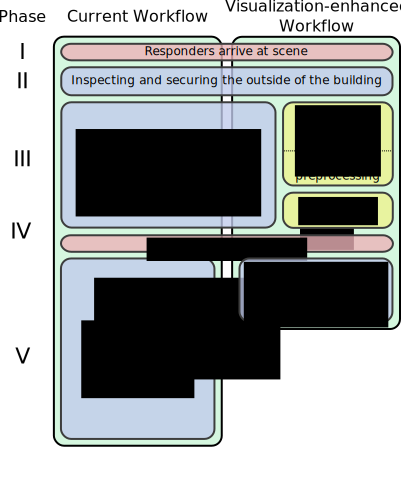
\includegraphics[width=0.9\columnwidth]{figures/workflow.pdf}
	\caption{A schematic timeline overview of the currently employed workflow (left) and our proposed visualization-enhanced system (right), showing all events (red) and actions (blue) split up into five distinct phases (roman numerals). Utilizing the additional actions (yellow) in parallel and thus enabling faster and less dangerous exploration, we decrease the overall time-to-rescue.}
	\label{fig:workflow:workflow}
\end{figure}

\begin{figure}[b]
    \vspace{-0.2cm}
	\centering
	\fbox{\includegraphics[width=0.6\columnwidth]{figures/map-drawing.jpg}}
	\caption{The currently employed workflow in search \& rescue operations requires the \IC\ to draw a 2D map by hand for orientation. The FEMA standards for annotations are visible in the lower part.}
	\label{fig:workflow:sota}
\end{figure}

While there is no general definition of a rescue team in an USAR incident, in most protocols, for example in FEMA~\cite{fema08} or Emergency Management Australia~\cite{em35}, one \IC\ is responsible for a single building and instructs multiple rescue responders inside this building. In this section, we will describe the current workflow first (see Figure~\ref{fig:workflow:workflow}, left) and then propose a visualization-enhanced workflow supported by our system (see Figure~\ref{fig:workflow:workflow}, right). Roman numerals in the text refer to the corresponding phases in the figure.

\noindent {\bfseries Current workflow.} After arriving at the disaster scene (Phase \texttt{I}), the first step for the responders is to explore and secure the area outside the collapsed building (Phase \texttt{II}). No rescuer is allowed to enter the building before it is secured, which can take an hour or more to finish (Phase \texttt{III}). Then, based on the gathered information, the \IC\ determines valid entry points into the structure and directs rescuers into the collapsed structure to perform reconnaissance (Phase \texttt{IV}). Using constant radio communication, the rescuer inside the building slowly advances and reports his progress to the \IC, who draws a 2D map (see Figure~\ref{fig:workflow:sota}) based on that information (Phase \texttt{V}). The rescuer enters the unknown building with unquantifiable risks, like gas leaks or dormant fires, inside. Not only is the 2D drawing of an unstructured 3D building insufficient and inaccurate, it also does not provide acceptable spatial awareness. This is clearly an example of opportunistic control, where decisions are made opportunistically based on feedback from the environment. The map is created as the rescuer proceeds, inhibiting higher levels of control in the beginning of the path. Although responders may recognize situations, decisions regarding the path are limited to the extent of the current exploration and to their view of the local environment. Initially, therefore, any RPD is restricted to the local environment. Global planning is limited further by the ability of responders to communicate relevant structural information accurately to the \IC, such as angles of turns, which cause hand-drawn maps to experience drift. This technique of opportunistic exploration has further limitations in that a faster and safer path might exist, but is not known to the rescuer or the \IC\ at that moment.

\noindent {\bfseries Visualization-enhanced workflow.} The initial phases \texttt{I} and \texttt{II} are the same as in the currently employed workflow. However, while the responders secure the building, which is the most time-consuming of the initial tasks, unmanned robots are released into the structure and start recording and measuring the inside of the structure and feeding back information to the \IC\ (see the parallel execution in phase \texttt{III}). The map data from multiple robots is co-registered in real-time and the \IC\ inspects the map and determines viable entry points into the structure combining the map information with real-world input. The robots' sensors are able to detect most signs of victims using thermal cameras and heart beat detectors~\cite{6027084, Wu12Eulerian}, but as these measurements are uncertain, both false positives and false negatives might occur. The same holds true for hazardous environments like fires, gas leaks, structurally unsafe areas, chemical spills, or radiation. The data retrieval and preprocessing can be done in parallel while securing the perimeter, so that all information is available when phase \texttt{IV} begins. Based on suggested or selected POIs, the system computes optimal paths through the generated map, which the \IC\ can use to direct the rescuers into the building. This reduces time-to-rescue (Phase \texttt{V}) as the rescuers do not need to explore the building to the same extent, but can proceed directly to the POIs. The proposed system applies RPD to the whole situation, extends the number of available cues and planning from local conditions (tracking and regulating) to higher ECOM levels.

When planning the access paths, a variety of factors must be taken into account. The responder must maintain a safe distance from hazardous environments, avoid overhanging structures, and the ground must be both stable and level. The uncertainty in the data, the varying requirements, and the invaluable expert knowledge of the \IC\ make it infeasible to derive an algorithm taking all these variables into account. Furthermore, as these variables are extracted from uncertain data, they are difficult to quantify and are subject to uncertainties. The \IC\ has to perform trade-offs to choose between alternatives, for example favoring a longer path that is faster to traverse over a more dangerous, shorter path. These requirements for expert knowledge, as well as the uncertainty, make the path selection a perfect example demonstrating how the human-in-the-loop paradigm benefits the decision-making.

While the \IC\ is instructing the rescuer to follow one chosen path, the rescuer feeds back new information, for example possible victims or new hazards. The \IC\ incorporates this information into the application to update the mapping information and paths. This is of high importance as features might not only have been missed by the robots, but detected features might change during the rescue operation. Fires can start or extinguish, subsequent structural collapses can make areas inaccessible, or debris is removed after the initial reconnaissance making previously inaccessible areas available. %Although we are designing a system lifting the decision-making to a strategic control, this bears an opportunistic element of planning in the COCOM-sense. However, the system has to support replanning in a strategic control mode to be able to adapt to changing environments.

%%%%%%%%%%%%%%%%%%%%%%%%%%%%%%%%%%%%%%%%%%%%%%%%%%%%%%%%%%%%%%%%%%%%%%%%%%%%%%%%%%%%%%%%%%%
%%%%%%%%%%%%%%%%%%%%%%%%%%%%%%%%%%%%%%%%%%%%%%%%%%%%%%%%%%%%%%%%%%%%%%%%%%%%%%%%%%%%%%%%%%%

\section{System Overview} \label{sec:overview}

Combining expertise in visualization, cognitive systems engineering, rescue robotics, and thorough discussions with domain experts, we determined a set of requirements that must be fulfilled to make our system useful for the \IC. We employed theories from sense-making and decision-making (see Section~\ref{sec:theory}) to guide the design of our system to fully support the \IC. The visualization components are designed to comply with these theories and have been tested in a user study with external domain experts as described in Section~\ref{sec:evaluation}.

The components should fulfill the following requirements, which we have derived from our discussions with the collaborating experts:

\begin{description}
\item[R1] The system must increase the \IC 's spatial awareness by allowing for interactive exploration of the collapsed structure.
\item[R2] The system must enable the \IC\ to interactively annotate the acquired data to react to changing circumstances in the structure.
\item[R3] The \IC\ must be able to inspect multiple access paths and be able to compare them and make trade-offs.
\item[R4] The system must provide the tools to select a globally optimal path and allow for its execution.
\end{description}

The proposed system employs multiple linked views to address these requirements (see Figure~\ref{sec:overview:system}). In order to fulfill requirement {\bfseries R1}, our system visualizes the acquired point cloud in an interactive manner that preserves occlusion and helps the \IC\ to form a consistent mental model of the structure. Within this visualization, the \IC\ can seamlessly annotate newly discovered entrances, hazards, POIs, and forbidden areas, thus fulfilling requirement {\bfseries R2}. To address requirements {\bfseries R3} and {\bfseries R4}, we integrate a visual representation of the different paths into the 3D visualization, and provide separate in-depth analysis tools.

The following subsections explain the individual components of our system. Before the acquired data can be used by our system, a preprocessing must be performed, which extracts derived data from the point cloud (Section~\ref{sec:overview:preprocessing}). Following the preprocessing, interactive data annotation is possible (Section~\ref{sec:overview:annotation}). Since the selection of an optimal access path based on a computed path ensemble is a central component of the system, we describe this computation process together with the employed comparison metrics in Section~\ref{sec:overview:pathcomputation}. The analysis of the path ensemble is described in the same section, while Section~\ref{sec:overview:3dvisualization} provides details on the considerations that went into designing the 3D visualization components of our system.

\begin{figure}
    \centering
    \framebox[\columnwidth][c]{
        \includegraphics[width=\columnwidth]{figures/fig-overview-system2.png}
    }
    \caption{A screenshot showing our system for a typical scenario. The right view allows for detailed inspection and navigation. Each view can be maximized to fill the entire screen for in-depth inspection.}
    \label{sec:overview:system}
\end{figure}


\subsection{Data Preprocessing} \label{sec:overview:preprocessing}
The data preprocessing employed by our system consists of two steps. First, the data is scan-converted to facilitate 3D visualization and path computation. Second, attributes coding spatial information are derived, which are later used during the path analysis.

\begin{figure*}
	\centering
	\subfigure[Hazard distance field]{
	    \includegraphics[width=0.475\columnwidth]{figures/fig-overview-hazardfield.png}
	    \label{fig:overview:precomputation:hazardfield}
	}
	\hfill
	\subfigure[Support field]{
	    \includegraphics[width=0.475\columnwidth]{figures/fig-overview-supportfield.png}
	    \label{fig:overview:precomputation:supportfield}
	}
	\hfill
	\subfigure[Occupancy field]{
	    \includegraphics[width=0.475\columnwidth]{figures/fig-overview-occupancyfield.png}
	    \label{fig:overview:precomputation:occupancyfield}
	}
	\hfill
	\subfigure[Height component of Size field]{
	    \includegraphics[width=0.475\columnwidth]{figures/fig-overview-sizefield.png}
	    \label{fig:overview:precomputation:sizefield}
	}
	\caption{Attributes derived in the data preprocessing stage with values mapped to the colors of individual voxels. Colormaps are shown beneath the respective images. (a) distance to the closest hazard. (b) level of support. (c) occupancy or data density. (d) availability of space above each voxel.}
    \label{fig:overview:precomputation}
\end{figure*}

\noindent {\bfseries Scan conversion.} The data retrieved from the unmanned robots are an unstructured 3D point cloud of an affected building's interior. The resolution of the scan is highly dependent on the allotted scanning time as well as the employed scanner. One issue with directly rendering such point clouds is missing occlusion information and the non-uniform distribution of measured points. To avoid this problem, we perform a binning of the point cloud to obtain a three-dimensional voxel data structure on a regular grid. The voxel size is dependent on the scan resolution of the robot, as it is a trade-off between resolving smaller details and increasingly noisy data. In our cases, voxel sizes of about 5\,cm were considered to be sufficient with regard to this trade-off. While this is currently a user-specified parameter, we are positive that in the future, automated analysis techniques together with the knowledge of the scanning protocol will lead to an automatic derivation of this quantity. After the binning has been performed, the resulting grid-based data structure contains one voxel for all bins where the occupancy exceeds a certain threshold. In our approach, we discard every voxel that only depends on a single measurement point, since this is likely due to measurement noise. From this point on we call a measurement in the original point cloud a \emph{point} and refer to a position in the grid-based, binned point cloud as a \emph{voxel}.

\noindent {\bfseries Attribute derivation.} In the second part of the preprocessing, derived attributes are computed for the voxel data, which are subsequently used to determine a set of viable rescue paths and to support the analysis of these paths. We compute a \emph{hazard distance field} (Figure~\ref{fig:overview:precomputation:hazardfield}) that denotes the distance to the closest hazard points for each voxel, weighted by severity. Let $\mathbf{i}$ be the current voxel, $H$ the set of hazard points, and $H^{\mathbf{i}}_s$ the normalized severity for $\mathbf{i}$. The hazard field is given by: $h(\mathbf{i}) = \min_\mathbf{j}(\mathrm{L}_2(\mathbf{i}, H^\mathbf{j}) \cdot H^\mathbf{j}_s)$. The \emph{support field} (Figure~\ref{fig:overview:precomputation:supportfield}) shows the available supporting area for each voxel. This value determines whether there is enough floor available for a responder to walk without hindrance. The voxel neighborhood in the plane perpendicular to the gravity axis is considered as that plane coincides with horizontal surfaces. The \emph{occupancy field} (Figure~\ref{fig:overview:precomputation:occupancyfield}) denotes the number of  points each voxel is based on. A higher occupancy means that the voxel contains more points in the original point cloud data and thus provides a higher certainty. The occupancy can be increased by longer scan rates and better scanning technology. The \emph{size field} (Figure~\ref{fig:overview:precomputation:sizefield}) shows for each voxel if a rescuer can fit into the space above without squeezing. We calculate two size values, one with the rescuer standing up, and a second while crouching. However, the system is designed in such a way that different geometries, for example rescue robots, can be easily integrated during runtime as long as the defined geometry supports fast point-intersection tests. 

To compute viable paths, we also need orientation information to be able to exclude paths that would be too steep for a rescuer. We utilize data normals in order to indicate the orientation of structures of interest. We investigated two sensible measures for determining the normal direction at each voxel. In the first method we compute the least-squares fitted plane based on all the points in the original point cloud which are covered by a voxel. The normal of the resulting plane is used as the normal for the voxel. The second method performs a least-squares fit of the neighborhood of the voxel to determine the principal direction of the plane. In our tests we found that the first method results in greater stability provided higher occupancy, as they were less susceptible to measurement noise.


\subsection{Data Annotation} \label{sec:overview:annotation}
With respect to requirement {\bfseries R2}, it is essential for the \IC\ to be able to classify and annotate the data interactively. In our system, each voxel can belong to one of five classes. \emph{Unclassified} is the default type for all voxels and does not convey any special semantics. \emph{Start} voxels are entry points that are accessible and usable. This means that each path can start from any of these points. \emph{POI} voxels are denoted, either by the robots or by the \IC, to be destination points for a path. These could indicate that there is a potential victim or another mission-critical element at this location. \emph{Hazard} voxels have been declared as dangerous due to, for example, an ongoing fire or gas leak. Each hazard area has a normalized severity that denotes how dangerous it is. \emph{Forbidden} voxels can only be declared by the \IC\ and are areas completely out of reach for traversal. These points are used when, for example, a corridor collapses and is not accessible anymore.

The \IC\ can modify the classification for each voxel by directly interacting with the point cloud visualization using the mouse. He can either modify a single voxel or perform a radius-based selection of all nearby voxels close to the selection. This modification can be either removing all voxels from a classification, adding voxels to a classification, or removing selected voxels.


\subsection{Path Computation} \label{sec:overview:pathcomputation}
%\begin{table*}[bt]
%\centering
%\begin{tabular}{|c||c|c|c|p{5cm}|}
%\hline
%Attribute & Validity & Application & Type & Explanation \\ \hline
%Path Length & Path & Selection \& Path Computation & number & The overall length of the path in standard units\\ \hline
%Minimal Hazard Distance & global & Selection & number & The closest distance in standard units the path has to all hazardous areas \\ \hline
%Average Hazard Distance & global & Selection & number & The average distance in standard units the path has to all hazardous areas \\ \hline
%Maximum Hazard Distance & global & Selection & number & The maximal distance in standard units the path has to all hazardous areas \\ \hline
%Standard Deviation of Hazard Distance & global & Selection & number & The standard deviation of the distance to all hazard areas \\ \hline
%Hazard Distance & local & Selection \& Path Computation & number & The distance to the closest hazard for a particular point on the path\\ \hline 
%Minimal Support & global & Selection & number & Expl \\ \hline
%Average Support & global & Selection & number & Expl \\ \hline
%Maximal Support & global & Selection & number & Expl \\ \hline
%Standard Deviation of Support & global & Selection & number & Expl \\ \hline
%Support & local & Selection \& Path Computation & number & Expl \\ \hline
%Minimal Path Inclination & global & Selection & number & Expl \\ \hline
%Average Path Inclination & global & Selection & number & Expl \\ \hline
%Maximal Path Inclination & global & Selection & number & Expl \\ \hline
%Standard Deviation of Path Inclination & global & Selection & number & Expl \\ \hline
%Inclination & local & Selection \& Path Computation & number & Expl \\ \hline
%Size Restriction & local & Selection \& Path Computation & boolean & Expl \\ \hline
%\end{tabular}
%\caption{A list of all attributes which are used in this work alongside explanations.}
%\label{tab:attributes}
%\end{table*}

For the path computations, we employ the widely used A* algorithm~\cite{4082128}. It is a best-first search algorithm that uses the L$_2$ distance as a heuristic to estimate the distance to the target. The algorithm works as follows: For the current point $x$, the estimated remaining distance is calculated for all unvisited neighboring points $y_i$. This value is the sum of the cost to reach $x$, the cost to move from $x$ to $y_i$, and the estimated cost to reach the target from $y_i$. These points are inserted into a list and the point with the lowest cost is chosen as the next valid point. the current point is then removed from the list and marked as visited. For a comprehensive description of the algorithm we refer the reader to the book by Russel and Norvig~\cite{AStar}.

When computing a path with A*, a metric is used which determines the cost of moving from one point to its neighbor. Thus, it is possible to compute several optimal paths by changing this metric. While it is technically possible to change the metric during the computation run, we did not include this into our system as the resulting complexity in interaction would be prohibitive for usability. The metric that is used in our system is composed of several, weighted sub-metrics that are summed up to yield the following metric:

\begin{equation}
\begin{array}{r@{}l}
m = & \textrm{distance}(\mathbf{p},\mathbf{q}) + w_h \cdot \textrm{hazard}(\mathbf{q}) + w_s \cdot \textrm{size}(\mathbf{q}) + \vspace*{0.1cm} \\
  & w_n \cdot \textrm{normal}(\mathbf{q},\varphi) + w_{sup} \cdot \textrm{support}(\mathbf{q},n)
\end{array}
\end{equation}

%\begin{eqnarray}
%m & = & \textrm{distance}(\mathbf{p},\mathbf{q}) + w_h \cdot \textrm{hazard}(\mathbf{q}) + w_s \cdot \textrm{size}(\mathbf{q}) + \\
%  & & w_n \cdot \textrm{normal}(\mathbf{q},\varphi) + w_{sup} \cdot \textrm{support}(\mathbf{q},n)
%\end{eqnarray}

\noindent where $w_h$, $w_s$, $w_n$, and $w_{sup}$ are the weights that are varied between different runs of the path computation. $\mathbf{p}$ is the current voxel and $\mathbf{q}$ is the next voxel under consideration.

The function $\textrm{distance}(\mathbf{p},\mathbf{q})$ calculates the L$_2$ distance between points $\mathbf{p}$ and $\mathbf{q}$ with the result in standard units. Since different scanners produce point clouds in different coordinate systems, it is necessary to convert all input into a standard set of normalized units. $\textrm{hazard}(\mathbf{q})$ returns the hazard severity that is stored in the hazard field. $\textrm{size}(\mathbf{q})$ is a binary function that determines if there is enough space above the voxel $\mathbf{q}$ by constructing the required geometry (with respect to the gravity vector) and testing if there is an intersection with the geometry and another voxel. The $\textrm{normal}(\mathbf{q},\varphi)$ function computes the surface normal for $\mathbf{q}$ and returns a normalized, linear response between the maximum allowed deviation $\varphi$ and the gravity vector. The $\mathrm{support}(\mathbf{q},n)$ value is dependent on the number of supporting voxels in the area around the point $\mathbf{q}$ and is retrieved from the support field. This area depends on the voxel size and should cover an area of about 50cm to allow safe passage. The parameter $n$ is a threshold determining how many surrounding voxels are needed to consider $\mathbf{q}$ being supported.

For different parameter combinations, the optimal path from the entry points to the POIs is computed. Some combinations might result in invalid paths, for example if $w_h$ is set to $\infty$ and the only possible path passes through a hazard field. We immediately exclude those paths from further inspection. If there are multiple POIs the \IC\ can choose to compute paths that visit each of the POIs in turn. This results in the traveling-salesman problem, which can be solved heuristically~\cite{4569756}.

To facilitate the subsequent analysis, global information is calculated for each path. Each path segment provides information about the distance to the closest hazard, while the path stores the minimum, maximum, and average distance together with the standard deviation to allow for in-depth analysis by the \IC. Furthermore, the total length of the path is calculated. 


\subsection{Visual Path Analysis} \label{sec:overview:pathanalysis}

In order to enable informed trade-offs between all computed paths and final selection of one suitable path, it is essential to provide detailed information about the various paths in an easily interpretable way for the \IC . The \IC\ can use linked views to filter the large number of computed paths in order to make an informed decision about an optimal trade-off. As the exact details of these trade-offs depend on the specific situation and the experience of the \IC, we provide adaptive tools to filter and analyze the path attributes according to the information the \IC\ requests, like \emph{Path Length} versus \emph{Minimal Hazard Distance} or \emph{Maximum Path Inclination} versus \emph{Minimal Support}. In this respect, the employed views have been selected such that they support single and multiple path analysis, as well as single and multiple attribute analysis. In addition it is desirable in some cases to see how certain attributes vary over the extent of a path. By exploiting these views in an interactive manner, the \IC\ can make full use of his knowledge in a strategic decision-making scenario. In the following, we will describe the intended role in the path analysis process for each view, as well as the design considerations we have made in order to ensure that each view fulfills this role in an optimal manner. As the path analysis starts with a larger set of paths which is reduced until a final path is selected, views facilitating comparison of multiple global path attributes for several paths are usually taken into account in the initial analysis phase. Later on the expert usually takes into account how attributes vary locally along the paths for an interesting subset of paths.

\begin{figure*}
	\centering
	\subfigure[Profile Plot]{
	    \fbox{\includegraphics[width=0.31\textwidth]{figures/fig-analysis-profile.png}}
	    \label{fig:overview:analysis:profile}
	}
	\hfill
	\subfigure[Parallel Coordinates Plot]{
	    \fbox{\includegraphics[width=0.31\textwidth]{figures/fig-analysis-pcp.png}}
	    \label{fig:overview:analysis:pcp}
	}
	\hfill
	\subfigure[Scatter Plot Matrix]{
	    \fbox{\includegraphics[width=0.31\textwidth]{figures/fig-analysis-scatter.jpg}}
	    \label{fig:overview:analysis:scatter}
	}
	\caption{Several analysis views supporting comparative path analysis based on attribute combinations. (a) the Profile Plot presents the change of a single attribute along each path; here the distance to the closest hazard. (b) the Parallel Coordinates Plot shows correlations between attributes. (c) the Scatter Plot Matrix depicts the correlations of all derived attributes and allows for arbitrary comparisons.}
\end{figure*}

\subsubsection{Profile Plot} \label{sec:overview:analysis:profile}
In order to enable a detailed analysis of attribute changes along a particular path, we include a \emph{Profile Plot} (PP). This is a variation of a line plot showing the change of a single attribute along the path, enabling the \IC\ to spot outliers among the paths. This view makes it easy to compare the paths with regard to the chosen variable since minima and maxima over all paths are easy to detect. Furthermore, it allows the \IC\ to spot irregularities along the path due to measurement errors, which would present themselves as single spikes and possible shifts (see the violet line in Figure~\ref{fig:overview:analysis:profile}). Having the possibility to detect these spikes, it is possible to fix the measurement errors and come to a more accurate path description. Figure~\ref{fig:overview:analysis:profile} shows the attribute \emph{Hazard Distance} for a set of paths.

While a PP is a simple line plot, several design considerations have been made to ensure effective use in the addressed scenario. First, a PP is meant as a link between the 3D path rendering and the more abstract visualizations enabling attribute comparison. Therefore, the paths are shown with their length on the x-axis and their color being the same as used in the 3D rendering. Thus, each line in the PP can be easily identified as a path and directly linked to the 3D view. As typically multiple paths are shown in the PP, the end point of each path is emphasized with a dot that enables a more direct comparison of path lengths, even when several paths overlap. Finally, the scale of the y-axis of the PP has been chosen such that a better attribute value discrimination becomes possible in regions of high importance. This is achieved by splitting the y-axis into three distinct parts, a sub-linear, a linear, and a super-linear part, which results in a focus-in-context representation. The splitting occurs around values of importance and enables the \IC\ to deemphasize less important value ranges, while providing a higher dynamic range on the y-axis to important values. We use the following mapping function

$$
f(x) = \left\{
    \begin{array}{ll}  
    l^{1-f} \cdot x^f & \textrm{if } x < l \\
    x & \textrm{if } l \leq x \leq u \\
    \frac{(u-1) \cdot \left( x^\frac{1}{f} - 1\right)}{u^\frac{1}{f} - 1} + 1 & \textrm{if } u < x
    \end{array}
    \right.
$$
to create a $C^0$-continuous mapping of a value $x \in [0,1]$ with a lower bound $l$, an upper bound $u$, and a exaggeration factor $f$. This yields a mapping that is sub-linear in $[0,l]$, linear in $[l,r]$, and super-linear in $[r,1]$. Figure~\ref{fig:remapping:factor} shows the mapping for a varying exaggeration factor.

An example of this remapping can be found in Figures~\ref{fig:remapping:original}~and~\ref{fig:remapping:modified}, which show the \emph{Hazard Distance} on the y-axis. For this attribute there is a non-linear importance of the value range. This means for the unmodified plot (\ref{fig:remapping:original}), that the important values are in the lower $\frac{1}{4}$ of the plot with the majority of the space wasted to less important values. Figure~\ref{fig:remapping:modified} shows the same values with the remapping function applied to the value range, providing higher detail for the important value differences. In addition the \IC\ can toggle a transparent layer in the PP to further highlight the important value range. The transparency of the layer is proportional to the amount of mapping that was performed: $\alpha(x) \propto 1 - \left| x - f(x) \right|$. To suppress an additional gradient that would draw unwanted attention at values 0 and 1, we clamp the $\alpha$ value to the range $[0.2,0.8]$.

\begin{figure}[b]
\vspace{-0.2cm}
\centering
\subfigure[The effect of the exaggeration factor $f$] {
    \includegraphics[height=0.265\columnwidth]{figures/remapping-function.png}
    \label{fig:remapping:factor}
}
\hfill
\subfigure[The unmodified Profile Plot] {
    \includegraphics[height=0.265\columnwidth]{figures/pp-original.png}
    \label{fig:remapping:original}
}
\hfill
\subfigure[Modified Profile Plot] {
    \includegraphics[height=0.265\columnwidth]{figures/pp-modified.png}
    \label{fig:remapping:modified}
}
\caption{The mapping function used in \emph{Profile Plots} emphasizes important ranges as a focus-in-context method. (a) the impact of multiple exaggeration factors $f$ for constant values of $l=0.4$ and $r=0.6$. (b) the original profile plot, while (c) a modified plot with values $l=0.025$, $u=0.275$, $f=0.1$.}
\label{fig:remapping}
\end{figure}

\subsubsection{Parallel Coordinates Plot} \label{sec:overview:analysis:pcp}
Figure~\ref{fig:overview:analysis:pcp} shows the \emph{Parallel Coordinates Plot} (PCP) of our system where each computed path is represented by a colored line. PCPs are a powerful visualization technique for the inspection of several multi-parameter data sets. They are very well suited to detect regularities and patterns in the data, deviations from these patterns, and also to enhance interactive exploration of data sources~\cite{Tory05aparallel}.

In our system, the PCP axes show the derived global path attributes, for example \emph{Path Length}, \emph{Minimal Hazard Distance}, \emph{Average Hazard Distance}, or \emph{Standard Deviation of Support}. The \IC\ can select which attributes are visible in the PCP, but the system provides a default view. Through attribute exploration, the \IC\ can move from a mental simulation of alternatives to simulation supported by the decision support system, thus amplifying RPD. The ability to explore trade-offs between alternative paths should facilitate a strategic COCOM decision mode for the targeting ECOM level. In addition to filtering of paths, which is replicated in all other views including the 3D rendering, the \IC\ can select a path in this view and the selection is likewise linked in the system. Detecting previously unknown correlations and the ability to filter large parts of the data helps to fulfill requirements {\bfseries R3} and {\bfseries R4}.

To ensure that the PCP can be used in an effective manner, we have taken into account several design considerations. One important aspect is to avoid confusion that might be introduced through the visual linking of the facilitated views. While using the same colors for the same paths supports mental registration in the different views, we ensure that this linking does not result in a direct matching of the paths. In the PP the x-axis represents the path length. Accordingly a line in the plot can be directly matched with the corresponding spatial representation in the 3D visualization; this is not the case for the PCP. While in the PCP a path is depicted as a line, the line does not support any spatial inference. Therefore, we have chosen to avoid the horizontal layout usually adapted in PCPs and rotate the PCP by 90 degrees to break the visual linking. Furthermore, we have chosen the ordering of the attribute axis as being fixed in a way that reflects the mental simulation of the \IC\ and their importance with respect to the path selection process. As the vertically oriented PCP is most likely to be read from top to bottom, the most important variables are displayed on the top of the plot. We have identified \emph{Path Length} and \emph{Minimal Hazard Distance} as the most crucial attributes for the path finding. These are shown on top. To enable an intuitive understanding of the different path attributes, we have ordered each axis in such a way that the preferable values are on the left, for example short \emph{Path Length} or a large \emph{Minimal Hazard Distance}. This results in a path layout where paths of high interest are located on the left.

Arranging the \emph{Minimal Hazard Distance} in the second row, enables direct semantic grouping with the other hazard-related attributes, which also have been sorted with respect to their importance from top to bottom. While all attributes are crucial to find a possible access path, the support-related attributes indicate how comfortable it would be to choose the selected path. Here we assume that it can be considered comfortable for a human to take a path if the support is above 50\,cm. To indicate that values below 50\,cm are not advisable, we mark out the value range between 0\,cm and 50\,cm. Since the actually needed support depends on several parameters, for example the fitness of the rescuer, we have decided not to discard paths based on this parameter but instead apply this masking procedure to leave the final decision to the \IC .


\subsubsection{Scatter Plot Matrix} \label{sec:overview:analysis:scatter}
The PCP is primarily used for aspects that we foresee that the \IC\ wants to compare frequently. However, in line with the literature on resilience engineering~\cite{Lundberg2012} we also provide comparisons that cannot be foreseen in advance. Therefore, we present the attributes additionally in a Scatter Plot Matrix (SPLOM), where each attribute is given by a row of scatter plots that show relations to all other attributes. It enables the \IC\ to make comparisons opportunistically by zooming in on the required comparisons if needed. Each individual scatter plot shows the correlation between two attributes and can be used by the \IC\ to verify known relationships or discover new correlations and interactions~\cite{Li2008}. In addition, paths selected in this view are linked to the other views providing a consistent representation of the available paths. Figure~\ref{fig:overview:analysis:scatter} shows the SPLOM during use. By using an identical color scheme in the scatter plot and all other plots, the \IC 's mental registration is not broken and he can intuitively use all plots to compare the available paths.


\subsection{3D Visualization} \label{sec:overview:3dvisualization}
\noindent {\bfseries Point cloud visualization.} Rendering the unfiltered point cloud proved to be insufficient in early tests, as wrong depth cues due to missing surface occlusion inhibited the necessary immersion in the scene. A voxelized representation is beneficial, as rendering each voxel using axis-aligned boxes solves the occlusion problem (Figure~\ref{fig:teaser}(a-c)). Holes appear in the rendering only in cases of very sparse data. To further increase the spatial awareness, we apply a shading technique to the rendering, where the lighting is based on the normal of the box's faces, rather than the computed voxel normal (see Section~\ref{sec:overview:preprocessing}). We use the face normal, as it is completely stable and constant for a given surface, thus making these surfaces easier to detect. As a second, optional, rendering method, we provide a simulated depth image that uses the normalized depth as a color scheme. This method resembles the output of range imaging cameras \IC\ are already familiar with. In order to deal with occluding objects, like a roof covering a building, the \IC\ can add and interactively modify clip planes.

\noindent {\bfseries Access path visualization.} In order to understand the paths' spatial relationship, it is desirable to show the paths embedded in the 3D visualization. Since the paths are computed based on the center points of the voxels, it is necessary to lift each path control point by at least half the voxel size in the opposite direction of the gravity vector. In our experiments, we found that raising paths by about two to three times the voxel size produces good visual results without paths looking too detached. Figure~\ref{fig:teaser}~(a-c) show paths that are rendered with an offset of three times the voxel size. To inhibit distracting discontinuities along the paths, we use the computed voxel centers as control points for a Catmull-Rom spline, which is rendered instead of a direct line connecting the voxel centers. 

In addition to using the same color as the other visualizations for each path, the \IC\ can select a different coloring scheme to inspect the stored attributes of the paths. Each path attribute can be mapped to the path segments for a quick visual analysis. Since the 3D visualization tends to become cluttered, we enable the user to select paths in the 3D visualization, which results in highlighting these paths in the linked views and desaturating all other paths. Thus, it becomes possible to inspect the behavior of a few paths without distraction, enabling the user to reduce the number of considered paths very quickly.

While our generated 3D visualizations have the benefits of being familiar to the \IC s, who are accustomed to working with 2D maps, 3D also enables entirely new ways of exploration. Rather than relying on a mental simulation of the situation, the \IC\ can use the visualization for a virtual walk-through to inspect whether a plan might actually work. This walk-through can either be steered by the \IC\ , or the camera follows a selected path automatically. By inspecting this information, the \IC\ can use his own experience to judge whether a path is feasible.

%%%%%%%%%%%%%%%%%%%%%%%%%%%%%%%%%%%%%%%%%%%%%%%%%%%%%%%%%%%%%%%%%%%%%%%%%%%%%%%%%%%%%%%%%%%
%%%%%%%%%%%%%%%%%%%%%%%%%%%%%%%%%%%%%%%%%%%%%%%%%%%%%%%%%%%%%%%%%%%%%%%%%%%%%%%%%%%%%%%%%%%

\section{Implementation} \label{sec:implementation}

%In this section, we describe the details necessary to reproduce this work. %We used the OpenMP framework~\cite{660313} for most of the preprocessing and path computation and achieved a speedup that is very close to linear.

\noindent {\bfseries Data preprocessing.} The input data is the acquired and co-registered point cloud from the autonomous robots~\cite{KohlbrecherMeyerStrykKlingaufFlexibleSlamSystem2011}. Each point in the point cloud stores its position in a global coordinate system, as well as additional information, like a color value or results from other scanners. As the global coordinate system is scanner-dependent, a transformation into a common coordinate system with standard units has to be performed. We transform the point cloud in such a way that the longest, axis-aligned side is mapped to the range $[-1,1]$. The conversion factor is stored to be later able to convert measurements back into the SI system. Based on this data the voxel binning and filtering is performed. A user-defined voxel size in SI units is prescribed and the points of the point cloud are assigned to their closest voxel center. The number of points per voxel is the occupancy, as described in Section~\ref{sec:overview:preprocessing}. The filtering step removes all voxels with an occupancy below a predefined threshold; in our case 2. This generates a second point cloud containing only the valid voxel centers. In a subsequent processing step, all attribute fields are computed for the voxel point cloud, for example normals, size restrictions, or support. These operations are performed in parallel for each voxel and do not require any intercommunication, thus providing a near-optimal parallelization. For the Tohoku dataset with 35 million points, the full pre-computation takes between two and three minutes on a four-core machine with 3\,GHz. 

\noindent {\bfseries Path computation.} As described in Section~\ref{sec:overview:pathcomputation} we use the A* algorithm with the metric $m$ to generate an ensemble of paths. The parameters of the metric span a six-dimensional parameter space. We sample this space on a regular grid and compute a path for each parameter configuration. High parallelism is possible since all paths are computed independently of one another. The fields are calculated for each path and are stored alongside an ordered list of voxels, whereby for each voxel the sub-metric decision criteria are stored as well. We sampled the parameter space at about $10^5$ positions and the computations required about two minutes on a 3\,GHz four core machine. In our experiments we found that an increase to about $10^7$ positions did not yield a significant increase in usable paths as most paths started falling into distinct classes. Considering the trade-off between computational time and number of paths, we found about $10^5$ to be a good trade-off between computation time and sampling density for current machines. With respect to the parallelism, an increase in cores will lead to a linear decrease in computation time.

\noindent {\bfseries 3D visualization.} The 3D visualizations are generated based on the preprocessed point cloud using OpenGL 4. The positions of the occupied voxel centers are stored in a vertex buffer object and rendered with a single \texttt{glDrawArrays} command. The different fields (see Figure~\ref{fig:overview:precomputation}) are stored in VBOs and attached as vertex attributes. The vertex shader performs packing of these values to increase the performance when the vertices are pushed through the pipeline. Although this operation reduces the dynamic range for the fields to 8 bits, the visual difference is minimal. As the size of the binning is known, a geometry shader constructs the vertices for an axis-aligned bounding box around each center, thus rendering the front faces of the boxes without the need for additional storage on the GPU. With all optimizations we achieve frame rates of at least $20$\,fps for our datasets on a GeForce GTX 580 graphics card.

%%%%%%%%%%%%%%%%%%%%%%%%%%%%%%%%%%%%%%%%%%%%%%%%%%%%%%%%%%%%%%%%%%%%%%%%%%%%%%%%%%%%%%%%%%%
%%%%%%%%%%%%%%%%%%%%%%%%%%%%%%%%%%%%%%%%%%%%%%%%%%%%%%%%%%%%%%%%%%%%%%%%%%%%%%%%%%%%%%%%%%%

\section{Results} \label{sec:results}
\begin{figure*}
\centering
   \subfigure[A scanned construction site with an ensemble of paths leading away from a construction worker standing on the edge of the pit.] {
       \fbox{\includegraphics[width=0.3\textwidth]{figures/tower-case-path.png}}
    \label{fig:overview:case:tower}
    }
    \hfill{}
    \subfigure[An ensemble of paths calculated in the Bremen rescue arena, which is used to test the autonomy of search \& rescue robots.] {
        \fbox{\includegraphics[width=0.3\textwidth]{figures/rescue-case-path.png}}
        \label{fig:overview:case:arena}
   }
   \hfill{}
    \subfigure[An intermediate result of the path computation in the Tokohu application case showing three classes of paths through the structure.]{
        \fbox{\includegraphics[width=0.3\textwidth]{figures/fig-analysis-rendering.jpg}}
        \label{fig:overview:analysis:paths}
    }
    \caption{Our system's rendering component during use in the application case (a) and the two test cases (b) and (c). The filtered paths are shown into the 3D rendering to provide an increased spatial awareness. Different weights for hazards lead to distinct optimal paths to the POI.}
\end{figure*}


Since autonomous robots are not yet used in emergency situations as the required equipment would interfere with the rescue personnel, it is not possible to apply our system to datasets from a real-world disaster area. Instead, to illustrate the flexibility of our system, we describe the application to one major application case and two test cases.

\subsection{Test Cases} \label{sec:results:testcases}
\noindent {\bfseries Construction site.} Figure~\ref{fig:overview:case:tower} shows a rendering of a point cloud acquired at a construction site with a LiDAR scanner being inside an excavation pit. We resampled the original dataset consisting of $50$ million points to $3.5$ million voxels with a voxel size of 5\,cm. The pre-computation steps took about 3 minutes 30 seconds to complete on a 3\,GHz four-core CPU. This case was chosen to test how the system operates if a large reduction in points is performed.

\noindent {\bfseries Rescue arena.} Figure~\ref{fig:overview:case:arena} shows an ensemble of paths through the Bremen rescue arena~\cite{varsadan08}, which is used as an artificial collapsed structure to challenge autonomous robots. As this testing arena was build specifically for search \& rescue scenarios, it proved to be an invaluable test case to apply path finding and selection. The original point cloud consists of $28$ million points, reduced to $5.3$ million points with 4\,cm resolution. This computation took about 2 minutes to complete on the same machine as above.

\subsection{Tohoku Application Case} \label{sec:results:applicationcase}
\begin{figure}[b]
    \vspace{-0.5cm}
    \centering
    \subfigure[\emph{Standard Deviation of Support} in relation to the \emph{Path Length}] {
        \includegraphics[width=0.3\columnwidth]{figures/pathlength-stddevsupport.png}
        \label{fig:overview:analysis:lengthstddev}
    }
    \hspace{0.5cm}
    \subfigure[\emph{Average Hazard Distance} in relation to the \emph{Path Length}] {
        \includegraphics[width=0.3\columnwidth]{figures/pathlength-averagedistance.png}
        \label{fig:overview:analysis:lengthavg}
    }
    \caption{Two zoom-ins of the Scatterplot Matrix (Figure~\ref{fig:overview:analysis:scatter}).  (a) \emph{Standard Deviation of Support} and (n) \emph{Average Hazard Distance} in relation to the \emph{Path Length}.}
\end{figure}


The major use case to which we have applied our system is based on three scans from a collapsed building at Tohoku university in the aftermath of the 2011 earthquake in Fukushima. The resulting dataset has been acquired with latest state-of-the-art equipment and consists of $26$ million sampling points~\cite{journals/jfr/NagataniKOOYTNYKFK13}, which we resampled to a voxel grid of $4$ million voxels with a voxel size of 3\,cm. As there had been partial collapses in the office building, it proved to be a valid and useful simulated real-world application case to test our proposed system with respect to uneven ground and obstacles. Figure~\ref{fig:teaser:1} shows a closeup rendering of the data set, which shows that the level of detail is sufficient to support spatial awareness. The rendering clearly shows a room with a chair and a table visible on the right, shelves on the left and a window in the back wall.

Figure~\ref{fig:teaser:3} shows an overview of the scanned area with the selected entry area at the bottom in cyan and the POI in green at the top. No hazards were detected by the robots during the acquisition as this was not part of their mission profile. The task for this application case was as follows: the \IC\ needed to find the shortest path between the entry and the POI. While traversing the path, an imaginary rescuer would detect two hazard clouds (highlighted in red) and the system must be able to react to this changing situation as by requirement {\bfseries R2}.

In Figure~\ref{fig:overview:analysis:paths}, a subset of computed paths after the second hazard has been discovered. There is one class of paths (purple) that evades the first hazard and another class (green) that evades the second hazard. The parallel coordinates plot (Figure~\ref{fig:overview:analysis:pcp}) makes it possible to detect a path that belongs to both classes with a maximum in the \emph{Minimal Hazard Distance}, while having a long \emph{Path Length}. The scatterplot showing the relationship between \emph{Path Length} and \emph{Standard Deviation of Support} indicates that the shorter paths tend to pass through more unstable areas (see Figure~\ref{fig:overview:analysis:lengthstddev}). There are no paths available with low overall length and stable ground. The paths with the lowest length also have the highest standard deviation of the computed support value.

Likewise, the scatterplot of \emph{Path Length} and \emph{Average Hazard Distance} shows distinct classes; only one of those providing simultaneously an acceptable \emph{Path Length} and high \emph{Average Hazard Distance}. There are five distinct clusters which simplifies the path selection for the \IC . Only one cluster seems reasonable as it has simultaneously an acceptable path length as well as a long average distance to the hazard.

%%%%%%%%%%%%%%%%%%%%%%%%%%%%%%%%%%%%%%%%%%%%%%%%%%%%%%%%%%%%%%%%%%%%%%%%%%%%%%%%%%%%%%%%%%%
%%%%%%%%%%%%%%%%%%%%%%%%%%%%%%%%%%%%%%%%%%%%%%%%%%%%%%%%%%%%%%%%%%%%%%%%%%%%%%%%%%%%%%%%%%%

\section{Evaluation} \label{sec:evaluation}
We performed an evaluation of our system with a total of nine external experts originating from six different countries working in the field of Urban Search \& Rescue. Of these experts, five (A--E) are emergency responders, three (F--H) are researchers, and one (J) is a consultant for a national technical relief agency. As the goal of the study was to include as many international experts as possible, and being aware of their time constraints, we decided to create videos and images of our system for the application case and created an interactive webpage rather than requiring training for hands-on use of our system.

The private webpage exposed the experts to seven steps, each evaluating a specific component of our system. The experts had to read the instructions for each component, inspect images and/or videos and then reply to questions and give feedback. They could pause and resume the evaluation as often as they wanted, as there was no imposed time limit. 7 of 9 experts finished the evaluation and provided answers to all questions. One expert stopped the evaluation after step 3, while the second stopped after step 5. In the result analysis we have considered the partial responses for the cases where an answer was provided. The average time the experts took to finish the evaluation was 57 minutes and 47 seconds, excluding two experts who paused and resumed the evaluation with a significant delay of several hours. One outlier was expert F, who took 20 minutes 56 seconds to complete the tasks.

The feedback is grouped into four different categories; first, questions to let the expert assess his own knowledge about the specific  component. With these questions, we can estimate whether the expert has prior knowledge and how intuitive the visualization is. The replies to these questions are on a 5-point Likert scale. The second type of questions are factual checks that have a \emph{correct} answer. These are used to test if the expert's self-assessment is accurate. The third type of questions are open-ended and allow us to gain insight into the thinking process of the expert. Usually these questions are alternatives for which there is no best answer, but requiring trade-off and domain knowledge. The fourth type of response asks for general comments about a component. We asked the experts to be as elaborate as possible for these replies. The full evaluation and replies are available in the supplemental material. Here, we will highlight and discuss the most important positive and negative answers by the experts. 

\noindent \textbf{3D Representation} This component evaluates the general usefulness of the voxelized point cloud's 3D rendering. A video as well as images similar to Figures~\ref{fig:overview:analysis:paths},~\ref{fig:teaser:2}, and~\ref{fig:teaser:1} were provided in shaded rendering as well as simulated depth images. The experts were asked to rate the degree of immersion (average: 2.94), the level of knowledge they had acquired (average: 2.5), if the rendering was more useful than a birds-eye view (average 3.77), and if the 3D rendering was useful in general (average: 4.14). To test the level of immersion and knowledge of the scene, we asked the experts to describe the room shown in the images, which all performed successfully, leading us to believe that the experts underestimated the knowledge they gained from the 3D rendering. An outlier in the responses was expert F, who reported 1 for the knowledge and 5 for the usefulness, but described the room correctly. We assume the answers are related to his comment, asking us to ``improve [our] registration algorithm''. We will forward this feedback to the team that performed the scanning and registration of the data set. Experts F and J asked us to provide camera images in the rendering, which was unfortunately not available for this data set, but we plan to add this functionality in the future.

\noindent \textbf{Path Representation} This component tests the usefulness of embedding the paths into the 3D rendering. It shows three images depicting the same situation as Figure~\ref{fig:teaser:2} with three paths each. The first scenario with no hazardous areas, the second with the upper hazard only, and a third with both hazards. We asked the experts which of the paths they would choose. All but two (A and F) chose the paths that evaded the hazards. A and F flipped the answers for the second and third scenario, letting the rescuer, in scenario 2, take a long path without a hazard in the way, while for scenario 3 ignoring the hazard and sending him through the hazard. We assume this to be an input error. A second question was asked to compare the lengths of the shortest and the longest path. While the correct answer was 1.54x the length, the experts stated an average of 2.56x. This means that, while the experts are capable of estimating the length within a reasonable margin of error, they overestimate path distances, making it necessary to provide accurate information in the PP and PCP.

\noindent \textbf{Evacuation Path Walkthrough} In this component, we evaluated the combined effects of the first two components. We generated two camera paths from the longest path in component 2; one path moving from the \emph{Start} to the \emph{POI} and a second moving from the \emph{POI} to the \emph{Start}. We asked for the usefulness (average: 3.125) and the self-assessed knowledge (average: 2.75) for both paths. We then asked the experts to describe possible obstacles along the way and to look for similarities along the two paths. The expected outcome for this question was to realize that both paths are the same. Experts C and J detected similar structures in both videos but did not say unambiguously that they are the same structures. Expert J's description of the obstacles are detailed and he uses the same words to describe both paths, leading us to believe that he did in fact notice the path's identity. Experts A, F, and G did not provide feedback on the obstacles, but the remaining four detected the same classes of valid obstacles, for example rubble piles or problems concerning structural integrity. %Experts F and J repeated their valid requests for colored and textured data as it would help the understanding, the cognitive load, and orientation in the scene.

\noindent \textbf{Profile Plot} In order to evaluate the PP, we provided a reduced plot containing only the orange, green, and yellow paths from Figure~\ref{fig:overview:analysis:profile}. To reduce learning effects we used the colors blue, orange, and red instead. The three paths are the same as in scenario 3 of the second component. We asked the experts to assess their understanding of the plot (average: 3.5) and the usefulness (average: 3.71). Asking for the total number of paths, the shortest path, and the number of times it crosses the hazard area, all experts gave the correct results. For the next question, we asked the experts to relate the two longest paths to each other; six experts arrived at the correct conclusion that the orange path is shorter, but crosses the hazard area once and can therefore be considered as less safe. Expert A did not provide any answer and expert F thought the orange path to be safer than the red path.

\noindent \textbf{Parallel Coordinates Plot} The level of self-assessed understanding is significantly lower compared to the PP (average: 1.66 vs. 3.5) which can be attributed to the fact the experts might be familiar with line plots, but did not experience PCPs before. Nevertheless, previous research on PCP~\cite{CGF:CGF1666} and correct answers prove that the PCP can still be a valid and useful component in our system. Expert F answered to all questions that he was unable to read the plot. Despite their unfamiliarity, all five experts providing feedback answered the questions about the shortest and the safest path correctly, identifying the path with the lowest path length and the highest minimal distance. In the following open questions, the experts seemed to favor safe, long paths over shorter, more dangerous paths while not paying much attention (except expert J) to the available support. This confirmed our previous discussion about the fixed ordering of attributes in the PCP. The experts rated the usefulness of the PCP with an average of 2.14. 

%This component showed the same scatter plot as in Figure~\ref{fig:overview:analysis:scatter} and asked for the shortest and then the most stable path with regard to the distance to hazard.
\noindent \textbf{Scatterplot Matrix} For this representation, the very low level of self-assessed knowledge (average: 1.16) and usefulness (average: 1.28) is, just as the PCP, probably due to the fact that while some of the experts might be familiar with scatter plots, few, if any, have worked with SPLOMs before. Only expert J provided replies to the questions asking for the shortest and the most stable path with regard to the hazard distance, and provided the correct answer to the best path with respect to the \emph{Standard Deviation of Hazard Distance}. No expert found the shortest path which is probably due to the fact that the scatter plot for \emph{Path Length} vs \emph{Path Length} was not included---a fact that can be easily solved. A comment from expert E summarizes the result for the SPLOM component: ``[this] is more information than I would want to interpret during a SAR mission''. We believe the SPLOM can have a beneficial impact to multivariate analysis~\cite{6064985}, but given the experts' reluctance, we plan to make the SPLOM an optional component instead.

\noindent \textbf{Miscellaneous} For the last part, we asked the experts if it is ``helpful to display the paths and [if it] provides additional information'', to which most experts (C, D, E, F, and J) agreed. Expert D noted that the GUI should be more ``user-friendly and understandable'' and expert J said that ``not detected hazards like structural integrity get visible by the density of scan points''. To the question if they ``[would] like to use [the] system in addition, or as a replacement, to [their] current tools'', the experts B, C, E, F, and J were positive to using our system in addition to their current set of tools rather than of a full replacement. Expert C would like to use it after a ``period of experimentation'', while expert J sees the system as ``an addition which is warmly welcome''. The only negative comment was from expert D, which regards the system as too complicated. Expert J also suggested possibilities for future work, suggesting that the system needs to be more intuitive to allow rescuers, who do not work with SAR operations on a daily basis, to use the system to its full potential. As a next step, we plan to conduct an additional study to assess the amount of necessary training for the USAR personnel to be able to use our system effectively.

In conclusion, we received valuable feedback from the contacted experts and we can draw the conclusion that most experts liked the system and would like to use it as a decision-support tool alongside their current cache of applications. With the exception of the SPLOM component, the majority of experts were able to retrieve important data from our system and use it for their decision-making.

%%%%%%%%%%%%%%%%%%%%%%%%%%%%%%%%%%%%%%%%%%%%%%%%%%%%%%%%%%%%%%%%%%%%%%%%%%%%%%%%%%%%%%%%%%%
%%%%%%%%%%%%%%%%%%%%%%%%%%%%%%%%%%%%%%%%%%%%%%%%%%%%%%%%%%%%%%%%%%%%%%%%%%%%%%%%%%%%%%%%%%%

\section{Conclusions and Future Work} \label{sec:conclusion}
In this paper, we presented a comprehensive visualization system that optimizes the workflow of an incident commander when dealing with search \& rescue missions in cases where the initial reconnaissance of a collapsed structure is performed using unmanned robots. We analyzed the workflow from a visualization perspective and designed a linked, multiple-view system that allows the \IC\ to effectively annotate a 3D visualization of a filtered point cloud. Based on this enriched data, our system computes and analyzes an ensemble of rescue paths that are explored by the \IC . The resulting information is visualized for the \IC , who can then select a path that is an optimal trade-off according to his experience and knowledge. To investigate the usefulness of the proposed system we have conducted a study with expert users. The resulting positive feedback makes us confident that the proposed system has the potential to improve future search \& rescue planning missions. In addition, we presented a stereoscopic movie of the application case and the rescue arena data sets to an audience of approximately 100 researchers at an IEEE-sponsored conference on rescue robotics. We received positive informal feedback from these research experts on the rendering over the course of later discussions.

For future work, we like to perform a thorough in-use evaluation workshop with domain experts accompanying a real-world rescue scenario. This will provide us with valuable direct feedback to improve usability of the system. Furthermore, we plan to investigate the applicability of adaptive and stochastic sampling, like Monte-Carlo methods, on the high-dimensional parameter space for path computation.

%%%%%%%%%%%%%%%%%%%%%%%%%%%%%%%%%%%%%%%%%%%%%%%%%%%%%%%%%%%%%%%%%%%%%%%%%%%%%%%%%%%%%%%%%%%
%%%%%%%%%%%%%%%%%%%%%%%%%%%%%%%%%%%%%%%%%%%%%%%%%%%%%%%%%%%%%%%%%%%%%%%%%%%%%%%%%%%%%%%%%%%

%\acknowledgments{For the major case, we like to thank the IRIDeS, the CREATE, and the IRS institutes for their cooperation in retrieving three scans from the Fukushima Daiichi nuclear reactor in the aftermath of the 2011 meltdown.
%This work was partly supported by grants from the Excellence Center at Link\"oping and Lund in Information Technology (ELLIIT) and the Swedish e-Science Research Centre (SeRC), as well as VR grant 2011-4113. We would like to thank the external experts for taking their time to take part in the evaluation. The presented concepts have been realized using the Voreen framework (www.voreen.org).
%}

\bibliographystyle{abbrv}
%%use following if all content of bibtex file should be shown
%\nocite{*}
\bibliography{bibliography}

\end{document}
